\documentclass{article}
\usepackage[margin=1in]{geometry}
\usepackage[utf8]{inputenc}
\usepackage{mathtools}
\usepackage{enumitem}
\usepackage{fancyhdr}
\usepackage{chngcntr}
\usepackage{tikz}

\lhead{Evan Kohilas - z5114986}
\rhead{COMP3821 - Assignment 3}
\pagestyle{fancy}
\title{A17S1N3}
\counterwithin*{equation}{section}
\usepackage{parskip}
\begin{document}

\begin{center}
    \begin{LARGE}
        COMP3121\\
        Assignment 3\\
        A17S1N3\\
        \hrulefill\\
        Evangelos Kohilas\\
        z5114986\\
        \hrulefill
    \end{LARGE}

    \begin{large}
        By submitting this document you are confirming that all the answers are your work and are not take from any other sources unless clearly mentioned.
    \end{large}

\end{center}

\section*{Question 1}
let $lps$ be the largest path sum by traversing the largest branches of the tree.

We can then find the minimal tree by recursing down the tree and changing the path sum for the leaf nodes, and then reducing and merging the lengths as we move back up the tree. By reducing through merging, we can always create a tree of minimal weight while still having an equal path sum, as we would be reducing all unncessary lengths.

% new_length = min(node.right.length, node.left.length) - 1
def recurse(node):
    if node.left is leaf and node.right is leaf:
        new_length = max(node.left_length, node.right_length)
        node.left_length = new_length
        node.right_length = new_length
        return new_length
    else:
        node.left_length = recurse(node.right)
        node.right_length = recurse(node.left)
        return min(node.left_length, node.right_length)

\begin{verbatim}
recurse(node, lps, sum=0):
    if node is leaf:
        old_length = node.length
        node.length = lps - sum
        return old_length
    else:
        old_left_length = recurse(node.left,  lps, sum + node.left.length)
        old_right_length = recurse(node.right, lps, sum + node.right.length)
        new_length = max(old_left_length, old_right_length)
        node.right.length = new_length
        node.left.length = new_length
        old_length = node.length
        node.length += new_length
        return old_length
\end{verbatim}

\pagebreak
\section*{Question 2}
The objects should be machined in descending order of polishing time, and then ascending order of machining time.

\textbf{Proof of optimality:}\\
let $A$ be our greedy solution produced by our algorithm and $O$ be the optimal solution.\\
let $m, p$ be the machining and poilishing time of some item and $m', p'$ be the machining and polishing time another item.


In the case where $p' < p$ and $m' = m$, we let the time taken for two items done in order $a$ and $b$ be $a_m + b_m + \max(a_p - b_m, b_p)$

If $A$ selects $(m, p)$ to be machined first, we let $total_A = m + m' + \max(p - m', p')$

In the first case where $p > m$:
\begin{align*}
    total_{A}^1 &= m + m' + p - m'\\
              &= m + p\\
\intertext{Otherwise:}
    total_{A}^2 &= m + m' + p'\\
              &= 2m + p'
\intertext{%
If we violate our greedy choice and $O$ selects $(m', p')$ to be machined first,\newline
we let $total_O = m' + m + \max(p' - m, p)$\endgraf
In the first case where $p > m$:%
}
    total_{O}^1 &= m' + m + p\\
              &= 2m + p
\intertext{Otherwise:}
    total_{O}^2 &= m' + m + p' - m\\
              &= m + p'
\end{align*}

Then we see that $total_{A}^1 < total_{O}^1$ and $total_{A}^2 < total_{O}^2$.\\
Therefore the optimal solution $O$ is worse than the greedy solution $A$.

In the case where $p = p'$ and $m' < m$, we let the time taken for two activities done in order $a$ and $b$ be $a_m + \max(a_p, b_m + b_p)$

Using $A$, we select $(m, p)$ to be machined first, so we get:
\begin{align*}
    total &= m' + \max(p', m + p)\\
          &= m' + \max(p', m + p')\\
          &= m' + m + p'
\end{align*}

If we violate our greedy choice and $O$ selects $(m', p')$ to be machined first, we get:
\begin{align*}
    total' &= m + \max(p, m' + p')\\
           &= m' + \max(p, m' + p)\\
           &= m' + m + p
\end{align*}

Then we see $total = total'$ showing no difference between $O$ and $A$.

Since a change in machining time sees no difference, then there will be no difference in every other case.

Therefore, $A$ is optimal as we cannot create a better solution than the greedy one produced by our algorithm.

\section*{Question 3}
If Alice makes a graph connecting people that know eachother, Alice can continously remove all people of degree less than 5 until either everyone is removed (in which case the constraints cannot hold for any ammount of invitees) or until no more people can be removed (in which case the largest number of invitees have been found).

\textbf{Proof of optimality:}\\
let $S = {p_1, p_2, p_3, \ldots, p_n}$\\
let $O$ be the set of the optimal solution.\\
let $S_i$ be the subset of $S$ after $i$ iterations where $0 \leq i \leq n$.

We prove by induction that $O$ will always be a subset of $S_i$.

When $i = 0$, no people have been removed, and so $O$ remains a subset of $S_0$

Assume $i = k$ such that after $k$ iterations, $O$ is a subset of $S_k$

let $i = k + 1$:\\
$O$ will still remain as a subset of $S_{k+1}$ as $p_{k+1}$ will only be removed if $p_{k+1}$ doesn't satisfy the two constraints.

Therefore by induction, since $O$ is still a subset of $S$, $S$ is optimal since $|S| \geq |O|$ as we are trying to maximise the number of invitees.

\section*{Question 4}
\begin{enumerate}[label=\alph*)]
    \item
    Given the following arrangement,
    \begin{center}
    
\begin{tikzpicture}
        \tikzset{circles/.style={draw, circle, very thick, minimum size=5mm}}
        \node [circles, fill=black] (1) at (0, 0){};
        \node [circles, fill=black] (2) at (2, 0){};
        \node [circles]             (3) at (4, 0){};
        \node [circles]             (4) at (6, 0){};
        \node [circles, fill=black] (5) at (8, 0){};
        \node [circles]             (6) at (10,0){};
    \end{tikzpicture}
    \end{center}

    Then by using the closest pair method (the proposed algorithm) our total length will be $5 + 1 + 1 = 7$
    \begin{center}
    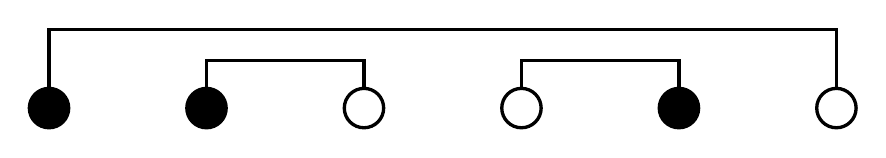
\begin{tikzpicture}
        \tikzset{circles/.style={draw, circle, very thick, minimum size=5mm}}
        \node [circles, fill=black] (1) at (0, 0){};
        \node [circles, fill=black] (2) at (2, 0){};
        \node [circles]             (3) at (4, 0){};
        \node [circles]             (4) at (6, 0){};
        \node [circles, fill=black] (5) at (8, 0){};
        \node [circles]             (6) at (10,0){};
        \draw [very thick] (1) |- +(0,  1) -| (6);
        \draw [very thick] (2) |- +(0,0.6) -| (3);
        \draw [very thick] (4) |- +(0,0.6) -| (5);
    \end{tikzpicture}
    \end{center}

    This is not optimal as the following solution has a shorter length of size $2 + 2 + 1 = 5$
    \begin{center}
    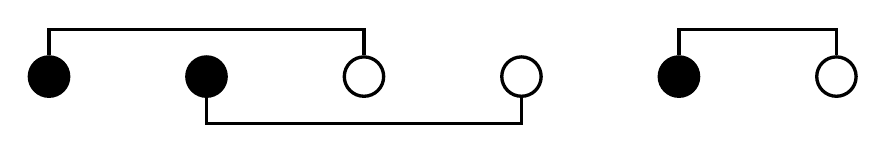
\begin{tikzpicture}
        \tikzset{circles/.style={draw, circle, very thick, minimum size=5mm}}
        \node [circles, fill=black] (1) at (0, 0){};
        \node [circles, fill=black] (2) at (2, 0){};
        \node [circles]             (3) at (4, 0){};
        \node [circles]             (4) at (6, 0){};
        \node [circles, fill=black] (5) at (8, 0){};
        \node [circles]             (6) at (10,0){};
        \draw [very thick] (1) |- +(0, 0.6) -| (3);
        \draw [very thick] (2) |- +(0,-0.6) -| (4);
        \draw [very thick] (5) |- +(0, 0.6) -| (6);
    \end{tikzpicture}
    \end{center}

    \item
        Going from left to right, each dot should be matched with its earliest possible matching dot.

        \textbf{Optimality Proof:}\\
        Let $A$ be our greedy solution produced by our algorithm and $O$ be the optiamal solution.

        If we violate our greedy algorithm, then there are two cases that can occur.

        If we swap two pairs in $A$ such that a pair finishes in the position of an earlier pair, then the earlier pair will finish in the position of the later pair, but the total length will not increase as both have been changed by the same amount.

        If we swap two pairs in $A$ such that a pair finishes in the position of a later pair, then the length of that pair will increase, but the length of the later pair will either decrease by an equal amount such that the total length will not increase, or not decrease, such that the total length has increased.

        Therefore, $A$ is optimal as we cannot create a better solution than the greedy one produced by our algorithm.

\end{enumerate}

\section*{Question 5}
To complete $n$ tasks with as low total penalty as possible, we pick the highest penalty task and schedule it to be completed as late as possible before incuring a penalty. If the picked task is scheduled to be completed in such a way that would incur a penalty, we ignore it, scheduling it to be completed after all tasks without penalty have been completed. We repeat this until all tasks have been scheduled.

\textbf{Optimality Proof:}\\
Let $A$ be our greedy solution produced by our algorithm and $O$ be the optiamal solution.

We can violate our greedy algorithm by swapping tasks from $A$ to $O$, such that they are either scheduled earlier, or scheduled later.

In both cases, by doing so we have either:
\begin{enumerate}
    \item Scheduled the tasks such that there is no change to the total penalty.
    \item Scheduled one of the tasks to be past its due date, and thus increasing our penalty.
    \item Scheduled a lower cost task to be before its due date, but sheduled a higher cost task after its due date, thus increasing out total penalty.
\end{enumerate}

Therefore, $A$ is optimal as all cases cannot create a better solution than the greedy one produced by our algorithm.

\section*{Question 6}
To calculate the first 10 books that we need to borrow, we iterate through the sequnce of books, adding each book to a set and continuing until our set is of length 10. Whenever we come across a book that is not in our set, we make another trip to the library, creating a new set and iterating as before.

\textbf{Optimality Proof:}\\
let $B$ be the sequence of books.\\
let $A$ be the set of the first 10 unique books from $B$ to keep produced by our algorithm.

Suppose $A$ is not optimal, and assume $O$ be the optimal solution.\\
If we violate the greedy algorithm then $|O| = 9$.

If $|O| = 9$ then one of two things have occured:

Either we have moved a book to the next set such as the next set will contain the $20^{th}$ book that we will need, as it will be the same as the book removed.

Or we have removed a book such that we require an additional trip to compensate for the $20^{th}$ book that could not be added to our set.

Therefore, $A$ is optimal as we cannot create a better solution than the greedy one produced by our algorithm.

\end{document}
